\documentclass[12pt]{article}
\usepackage[margin=1in]{geometry}
\usepackage{setspace}
\onehalfspacing

% Start of preamble
%==========================================================================================%

% Required to support mathematical unicode
\usepackage[warnunknown, fasterrors, mathletters]{ucs}
\usepackage[utf8x]{inputenc}

\usepackage[dvipsnames,table,xcdraw]{xcolor}

% Standard mathematical typesetting packages
\usepackage{amsmath,amssymb,amscd,amsthm,amsxtra}
\usepackage{mathtools,mathrsfs,xparse,newtxtext,newtxmath}

% Symbol and utility packages
\usepackage{cancel, textcomp}
\usepackage[mathscr]{euscript}
\usepackage[nointegrals]{wasysym}
\usepackage{apacite}

% Extras
\usepackage{physics}
\usepackage{tikz-cd}
\usepackage{microtype}
\usepackage{enumitem}
\usepackage{titling}
\usepackage{graphicx}

\usepackage{listings}
\usepackage{xcolor}

% Define custom colors
\definecolor{codebg}{HTML}{F8F8F8}
\definecolor{commentgreen}{HTML}{008000}
\definecolor{stringpurple}{HTML}{BA2121}
\definecolor{keywordblue}{HTML}{0000FF}
\definecolor{numbergray}{HTML}{666666}

% Enhanced Python listings settings
\lstset{
    language=Python,
    backgroundcolor=\color{codebg},
    basicstyle=\ttfamily\small,
    keywordstyle=\color{keywordblue}\bfseries,
    commentstyle=\color{commentgreen}\itshape,
    stringstyle=\color{stringpurple},
    numberstyle=\tiny\color{numbergray},
    numbers=left,
    stepnumber=1,
    numbersep=8pt,
    frame=single,
    framerule=0.5pt,
    rulecolor=\color{black!30},
    showspaces=false,
    showstringspaces=false,
    breaklines=true,
    breakatwhitespace=true,
    tabsize=4,
    captionpos=b
}

% Common shortcuts
\def\mbb#1{\mathbb{#1}}
\def\mfk#1{\mathfrak{#1}}

\def\C{\mbb{C}}
\def\R{\mbb{R}}
\def\Z{\mbb{Z}}
\def\cph{\varphi}
\renewcommand{\th}{\theta}
\def\ve{\varepsilon}
\newcommand{\mg}[1]{\| #1 \|}

% Often helpful macros
\newcommand{\floor}[1]{\left\lfloor#1\right\rfloor}
\newcommand{\ceil}[1]{\left\lceil#1\right\rceil}
\renewcommand{\qed}{\hfill\qedsymbol}
\renewcommand{\P}{\mathbb P\qty}
\newcommand{\E}{\mathbb{E}\qty}
\newcommand{\Cov}{\mathrm{Cov}\qty}
\newcommand{\Var}{\mathrm{Var}\qty}

% Sets
\usepackage{braket}

\graphicspath{{/}}
\usepackage{float}

\newcommand{\SET}[1]{\Set{\mskip-\medmuskip #1 \mskip-\medmuskip}}

% End of preamble
%==========================================================================================%

\title{CSE Template}
\date{\today}
\author{Rohan Mukherjee}

\begin{document}
    \maketitle
    \subsection*{Problem 1.}
    \begin{enumerate}[label=(\alph*)]
        \item They are all irreducible because from any starting state you can always reach any other by just walking around the cycle. On the other hand, the cycle with $n=17$ will indeed be aperiodic, since given any starting state $s$ we can reach it by walking forward 1 and back one, and then we can also walk around the entire cycle, which takes 17 steps. So the gcd divides 2 and 17 so it must be 1. Similarly, for the cycle with loops at even vertices, for even vertices we can walk around the self loop, which takes only 1 step, and on the other hand for odd vertices, we can walk forward and back, and also walk forward, loop at an even, and back, so it must divide 2 and 3 in this case and the gcd will be 1 always.

        For the odd length cycle (and in fact the even length one too), the vector $\pi = (1,\ldots,1)$ is a stationary measure, so normalizing it gives the stationary distribution. On the other hand, for the cycle with loops at even vertices, the stationary distribution will be $\pi = (2, 3, 2, 3, \ldots, 2, 3)$, since for one step of transition, the odd vertices have 2 paths to get to it, while the even vertices have the two cycle paths and the self loop, which gives slightly higher probability.
        
        However, the cycle graph with $n=18$ will not be aperiodic, since for any state $s$, $P^n(s,s) > 0$ only when $n$ is even, so the gcd will be 2 in this case.

        \item Here is the graph of the total variation distance for the three markov chains:
        \begin{figure}[H]
            \centering
            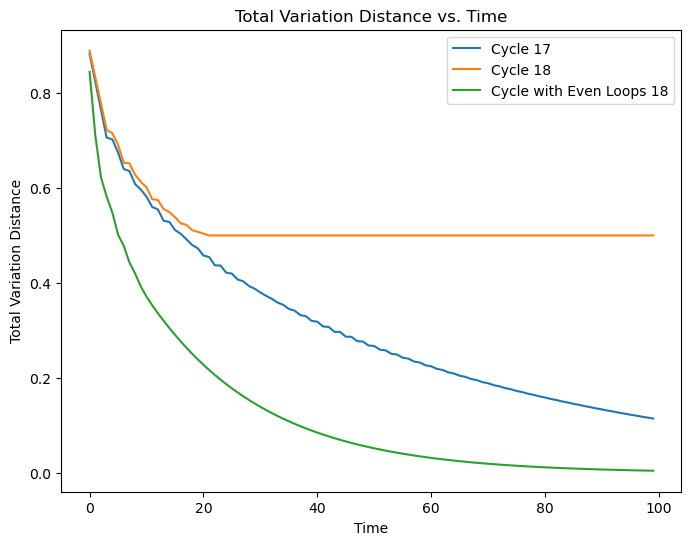
\includegraphics[width=0.7\textwidth]{tv.png}
        \end{figure}

        My code is as follows (as it turns out, for the only non-aperiodic chain, the stationary distribution will already be the uniform vector, so I don't have to manually change that):
        \begin{lstlisting}
def cycle(n):
    P = np.zeros((n,n))
    for i in range(n):
        P[i, (i-1)%n] = 1
        P[i, (i+1)%n] = 1
    return P/np.sum(P, axis=1, keepdims=True)

def cycle_with_even_loops(n):
    P = np.zeros((n,n))
    for i in range(n):
        P[i, (i-1)%n] = 1
        P[i, (i+1)%n] = 1
        if i%2 == 0:
            P[i, i] = 1
    return P/np.sum(P, axis=1, keepdims=True)

def stationary_distribution(P):
    eigenvalues, eigenvectors = np.linalg.eig(P.T)
    stationary_vector = eigenvectors[:, np.isclose(eigenvalues, 1)].flatten().real
    return stationary_vector / stationary_vector.sum()

def plot_mixing_time(P_list, labels=None):
    plt.figure(figsize=(8, 6))

    for i, P in enumerate(P_list):
        n = P.shape[0]
        stationary = stationary_distribution(P)
        distro = np.zeros(n)
        distro[0] = 1
        tvs = []

        for t in range(100):
            distro = distro @ P
            tvs.append(np.sum(np.abs(distro - stationary)) / 2)

        label = labels[i] if labels else f"Chain {i+1}"
        plt.plot(tvs, label=label)

    plt.xlabel('Time')
    plt.ylabel('Total Variation Distance')
    plt.title('Total Variation Distance vs. Time')
    plt.legend()
    plt.show()

plot_mixing_time([cycle(17), cycle(18), cycle_with_even_loops(18)], labels=['Cycle 17', 'Cycle 18', 'Cycle with Even Loops 18'])
        \end{lstlisting}

        \item Here are the eigenvalues: 
        \begin{table}[H]
            \centering
            \begin{tabular}{|c|c|c|}
            \hline
            \textbf{Graph Type} & \textbf{Second Largest Eigenvalue} & \textbf{Smallest Eigenvalue} \\
            \hline
            Cycle (17 vertices) & 0.9325 & -0.9830 \\
            Cycle (18 vertices) & 0.9397 & -1.0000 \\
            Cycle (18 vertices, self loops) & 0.9518 & -0.6667 \\
            \hline
            \end{tabular}
            \caption{Eigenvalues for different cycle graphs transition matrices}
            \label{tab:eigen_cycle}
            \end{table}

        \item The algorithm that we are running, which is to start with any distribution $\mu$ and then repeatedly do $\mu \leftarrow \mu P$, this is precisely the power method. The power method converges at a rate proportional to $\lambda_2/\lambda_1$. So smaller $\lambda_2/\lambda_1$ means faster convergence. However, you will notice above that the cycle with 18 and loops converges fastest, while having a bigger $\lambda_2/\lambda_1$ than the 17 cycle. Since our matrices are NOT PSD, I believe we need the absolute values of the eigenvalues to have large $\lambda_2/\lambda_1$, meaning if we order the eigenvalues like $|\lambda_1| \geq \ldots \geq |\lambda_n|$, we would want $|\lambda_1|/|\lambda_2|$ to be large. I believe, after accounting for them not being PSD, this is actually the quantity that shows up in the power method. For us, the largest eigenvalue is 1, while the second largest in magnitude is very large for the cycles, while smaller for the cycle with loops. This is why the cycle with loops converges faster. For non-PSD symmetric matrices, I believe it can get confused between the eigenvalues with equal magnitude, like we see in the regular cycle case, which causes it to take longer to decay. 

        \item From the above, we want a 3 regular graph that is extremely well connected. This is precisely the definition of an expander graph. I couldn't find a good expander graph, so I just sampled 100 random graphs and then picked the one with the largest $\lambda_1 - \lambda_2$, after some more research I think $\lambda_1/\lambda_2$ would've been better. Here is the graph it found:
        \begin{figure}[H]
            \centering
            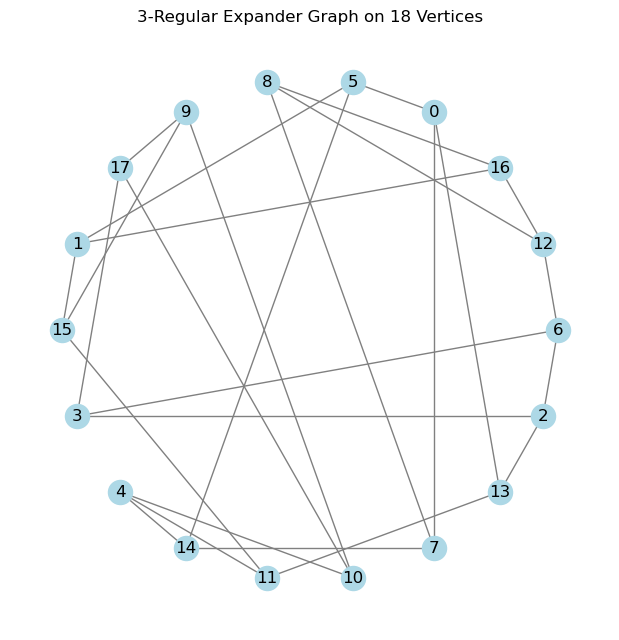
\includegraphics[width=0.7\textwidth]{random_graph.png}
        \end{figure}

        Here is its mixing time versus the other graphs:
        \begin{figure}[H]
            \centering
            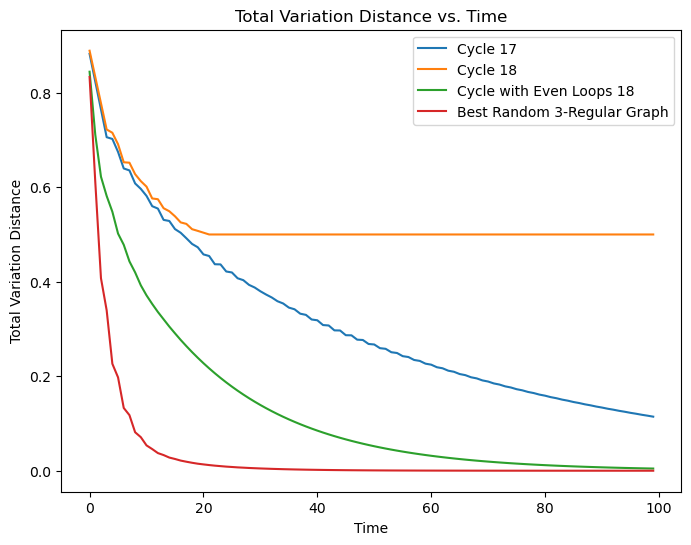
\includegraphics[width=0.7\textwidth]{tv_with_random_graph.png}
        \end{figure}

        Actually, I just realized that here I did MCMC too! MCMC on MCs!
    \end{enumerate}
    \subsection*{Problem 2.}
    \begin{enumerate}[label=(\alph*)]
        \item There are $30!$ states in our markov chain, the number of permutations on 30 parks. Our Markov Chain is irreducible, since given any other tour, we can do ``bubble sort'' to get to it, with each swap being a transition with positive probability (however, I believe this only holds with positive temperature, since if you are in the global minimum, it will have no outgoing edges. With positive temperature there is at least a positive probability to reach any of the neighbors that differ by only one consecutive swap, assuming they all have distinct tour lengths). So indeed, as $n \to \infty$, we will see every state a.s. (since our markov chain is finite, there is at least one recurrent state, so by irreducibility, all states are recurrent. So in fact we will see every state infinitely often).

        \item Here is the plot of the algorithms execution for $T \in \SET{0, 1, 10, 100}$:
        \begin{figure}[H]
            \centering
            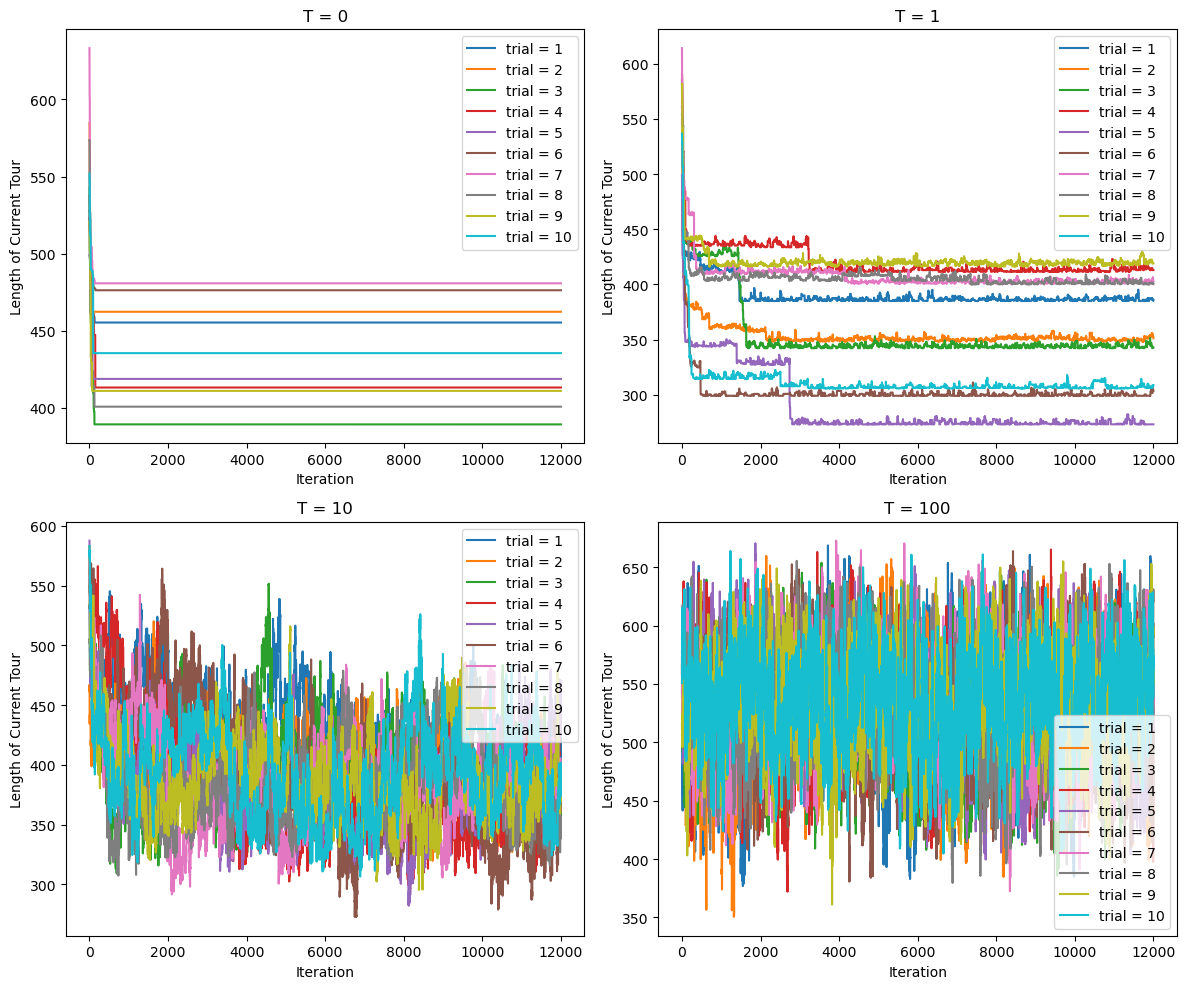
\includegraphics[width=0.8\textwidth]{alg.png}
        \end{figure}
        The best value of T here seems to be 1, it gets lower ending values for most executions than $T = 0$, while also sometimes being able to escape local mins, which $T = 0$ is just completely not able to do. $T = 10$ and 100 are way too high and just end up with extreme of volatility. 

        \item Here is the plot of the modified algorithm:
        \begin{figure}[H]
            \centering
            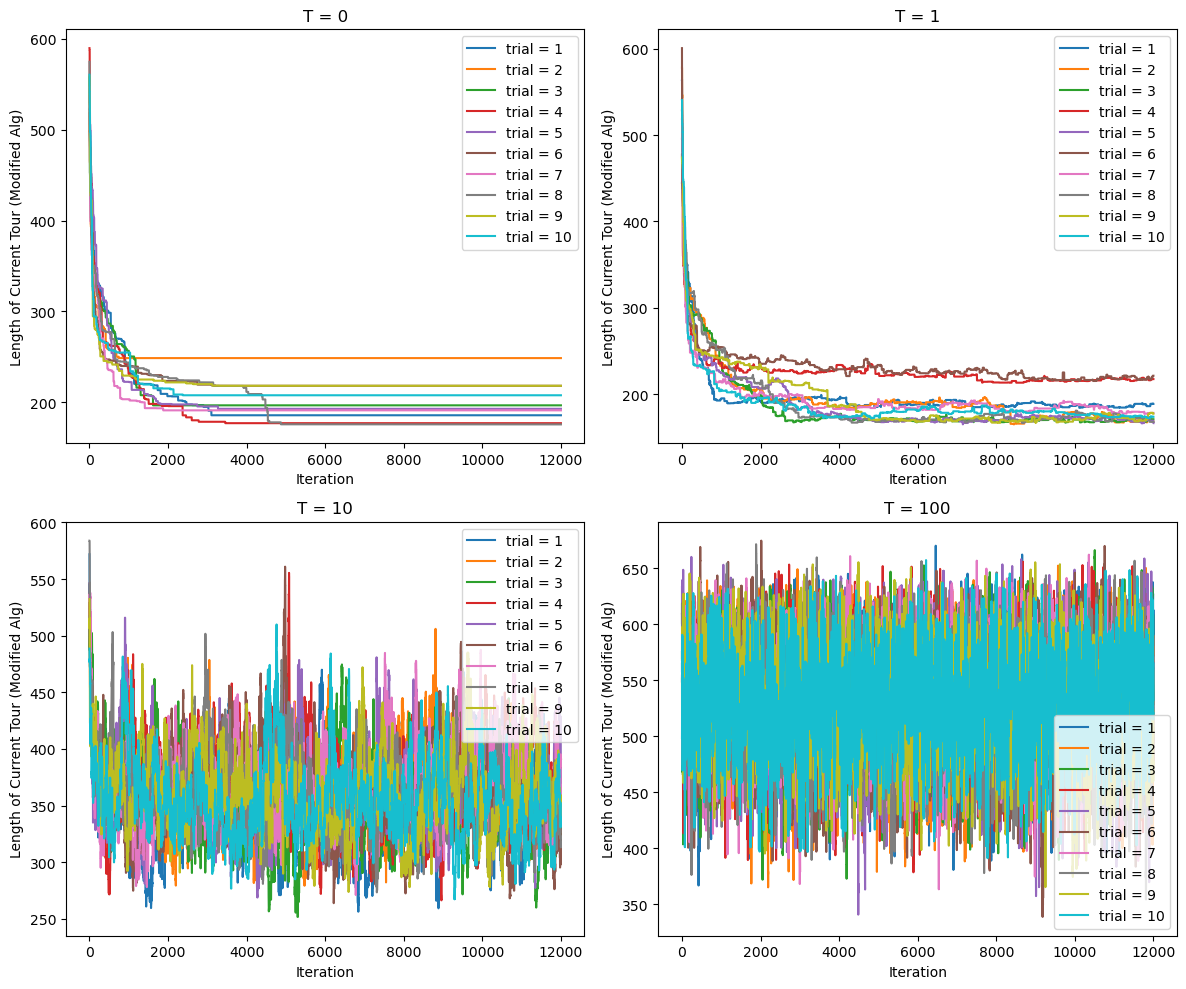
\includegraphics[width=0.8\textwidth]{modified_alg.png}
        \end{figure}

        Again the best value of $T$ here is 1 for the same reasons as above. It is pretty stable like $T=0$ but seems to get a lower tour cost on average (implying that it is a little less sensitive to the initial guess). 

        \item The best value of $T$ here seems to also be 1. Kind of shocking how bad $T=10,100$ are. Here, for $T=0,1$, the algorithm seems to take longer to converge, like 4000-6000 rather than 2000-4000. However, this modified algorithm also gets significantly better final values, down like 100-200 for both $T=0,1$. The spread on the iterations is significantly smaller for the modified algorithm than the original. From an anecdotal perspective, for the first algorithm, every vertex has degree $N$, so a local minimum is easier to achieve since you only have to be less than $N$ others. On the other hand, the modified has degree $N \choose 2$, so getting stuck in a local min is much harder. The problem also seems to be really sensitive to how good the initial guess is, with the last values being in the same order as the first values. From a mixing time perspective, the modified algorithm's graph would have clusters of size $N \choose 2$, so it would be fairly easy to color the graph since they are clustered up so well. There are clusters that are quite far away, and we would do good coloring each of these $N \choose 2$ clusters with different colors. On the other hand, the regular algorithm has only vertices of degree $n$, so this coloring strategy wouldn't work as well. From our interpretation with spectral graph theory, better colorings = higher $\lambda_2$, which in turn means smaller $\lambda_2/\lambda_1$. Smaller $\lambda_2/\lambda_1$ means it mixes slower. So we see the convergence of this second algorithm is much slower, however it still outperforms the first by quite a lot. This is most obviously seen with $T=0$, not allowing it to get stuck in local minima that quickly. 
        
        \item The difference between simulated annealing and this procedure is that the former decreases the temperature over time. As we saw, high temperature $T \geq 10$ is really bad over a long stretch of time. However, initally it will let the algorithm explore a lot more. We saw that the initial value is symbolic of the ending value. So the hope is that we can find a good initial value through a high temperature, then keep lowering it down so we can make the algorithm more stable. As we saw near the end, there isn't really a point in having high temperature as it just leads to microfluctuations. I would suspect simulated annealing to work much better, and in fact I believe this is how people do in RL (with initial high $\varepsilon$ and then it goes down) and with attention, and etc. It is just a good idea to shrink the exploration parameter over time.
    \end{enumerate}
\end{document}